\section{Capsule Cutting From the Cuboid with Bending}
The example is a capsule section cutting from the cuboid with bending as illustrated in fig.~\ref{oct_fig:ex_caplus_layout} and the corresponding mesh is illustrated in fig.~\ref{oct_fig:ex_caplus_mesh1.png}.
\begin{figure}[h!]
  \centering
  \scalebox{.5}{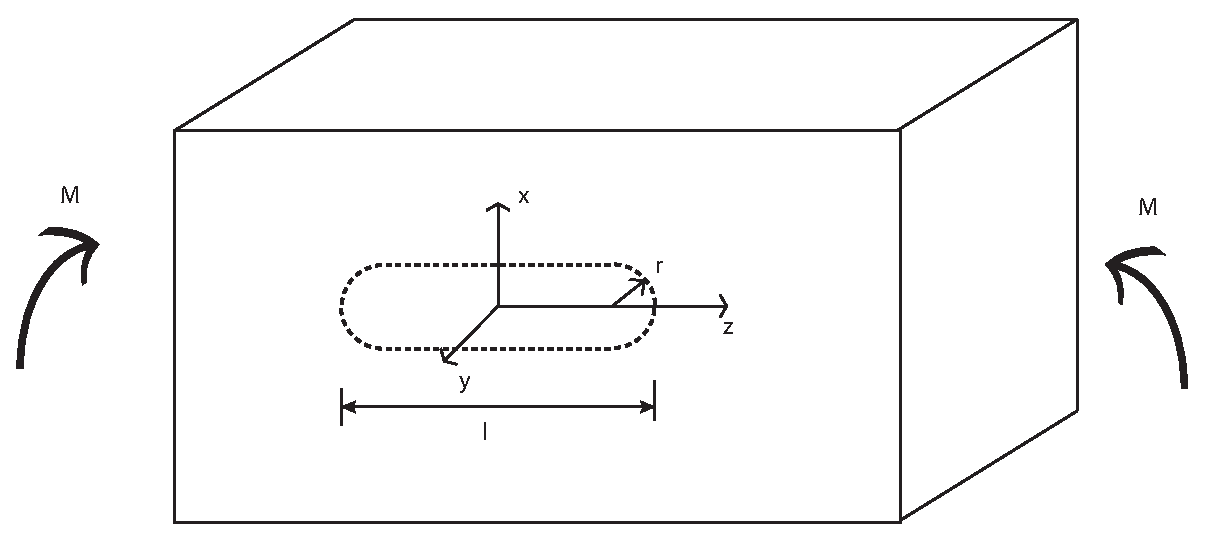
\includegraphics{octree/ex_images/oct_ex_caplus_rect.eps}}
  \caption{Problem layout}
  \label{oct_fig:ex_caplus_layout}
\end{figure}

\begin{figure}[h!]
  \centering
  \scalebox{.3}{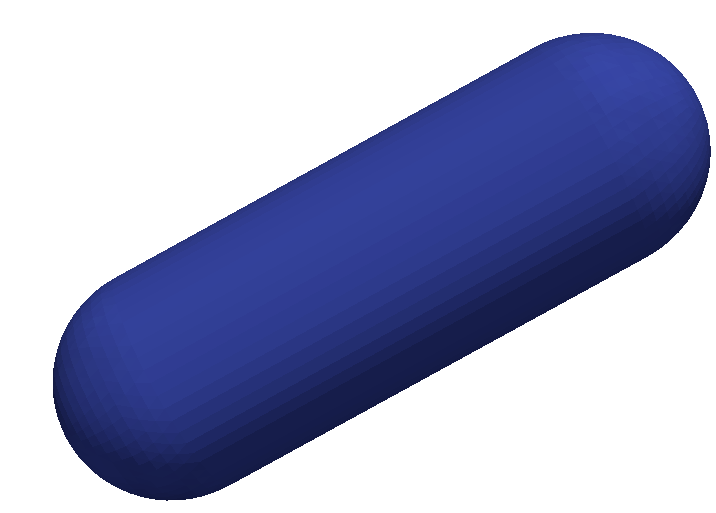
\includegraphics{octree/ex_images/oct_ex_caplus_geo.png}}
  \caption{Geometry of the capsule}
  \label{oct_fig:ex_caplus_geo}
\end{figure}


\begin{figure}[h!]
    \centering
    \begin{subfigure}[b]{1\linewidth}
        \centering
        \scalebox{.3}{
            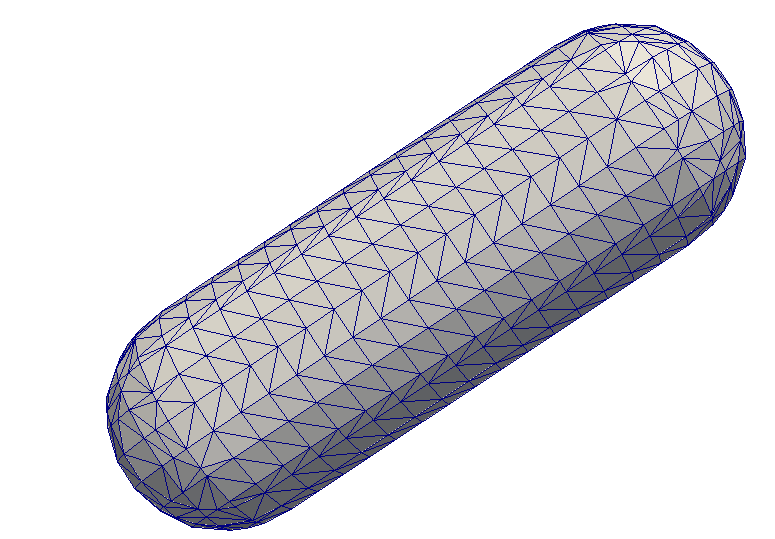
\includegraphics{octree/ex_images/oct_ex_caplus_mesh1.png}
        }
    \end{subfigure}
    \begin{subfigure}[b]{1\linewidth}
        \centering
        \scalebox{.3}{
            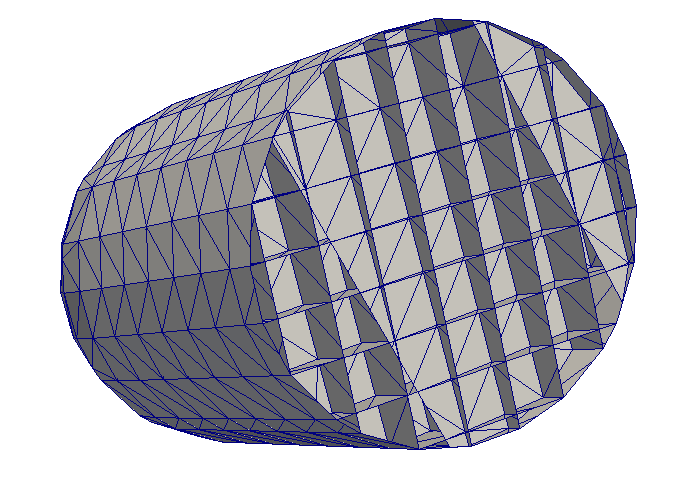
\includegraphics{octree/ex_images/oct_ex_caplus_mesh2.png}
        }
    \end{subfigure}
    \caption{Mesh of the Capsule}
    \label{oct_fig:ex_caplus_mesh1.png}
\end{figure}

The displacement analytical solution \cite{Tim1951} is applied on the outer surface of the capsule as the boundary condition and the displacement and stress (eqn.~\ref{eqn:caplus_stress}) inside is compared to the analytical solution. All stress component expect $\sigma_z$ is zero.
\begin{subequations}
\begin{align}
  u_x &= -\frac{1}{2R}\left[z^2 + \nu \left(x^2 - y^2 \right)\right]\\
  u_y &= -\frac{\nu xy}{R}\\
  u_z &= \frac{xz}{R} 
  \label{eqn:capluse_displacement}
\end{align}
\end{subequations}

\begin{equation}
  \sigma_x = \frac{Ex}{R}
  \label{eqn:caplus_stress}
\end{equation}

In the numerical calculation, The dimension of the outer cuboid will not affect the result because of the independence of the analytical solution (eq.\ref{eqn:capluse_displacement}). 6-nodes triangle element is used to achieve an exact solution. $l=100,r=17.5,\nu=0.2,E=30$. The error of the displacement are calculated as followed.
\begin{subequations}
\begin{align}
e_u &= \frac{||u_{ex} - u||}{||u_{ex}||}\\
e_s &= \frac{||\sigma_{ex} - \sigma||}{||\sigma_{ex}||}
\end{align}
\end{subequations}

The error of the displacement norm is $1.7563\times 10^{-14}$ and the error of the stress norm is $1.3184\times 10^{-9}$.
\pagebreak